\chapter{Rendering and Color Science}

This chapter serves as an introduction to the computer graphics and the color science. We briefly overview basic aspects of these fields, mainly to familiarize the reader with some of the fundamental processes, their backgrounds and usages. We also establish the terminology, such as \emph{rendering} or \emph{RGB color space}, that will be used throughout the thesis frequently. A significant part of the following sections is based on~\citet{wyszecki1982color},~\citet{nimier2019mitsuba} and~\citet{pharr2016physically}.

\section{Color perception}



\section{Physically based rendering}

One of the ultimate goals of the computer graphics is to be capable of reproducing visually plausible and physically coherent images based on a description of a scene that should be indistinguishable from a photograph of the same scene. Such process is called the \emph{photo realistic rendering}. In this thesis, we abbreviate the term and call it simply the \emph{rendering} as the non-photo realistic one does not concern us.

Depending on the implementation, the renderer simulates various phenomena commonly seen in nature such as light reflections, refractions, shadows, etc. Providing a powerful hardware, modern renderers adapt various physical models (or their approximations) of light transport or material properties to provide accurate photo realistic results. In reality, the renderers are so capable that the rendered images are almost indistinguishable from the real life photos. An example can be seen in \ref{fig:corona_render}.

\begin{figure}[H]
	\centering
	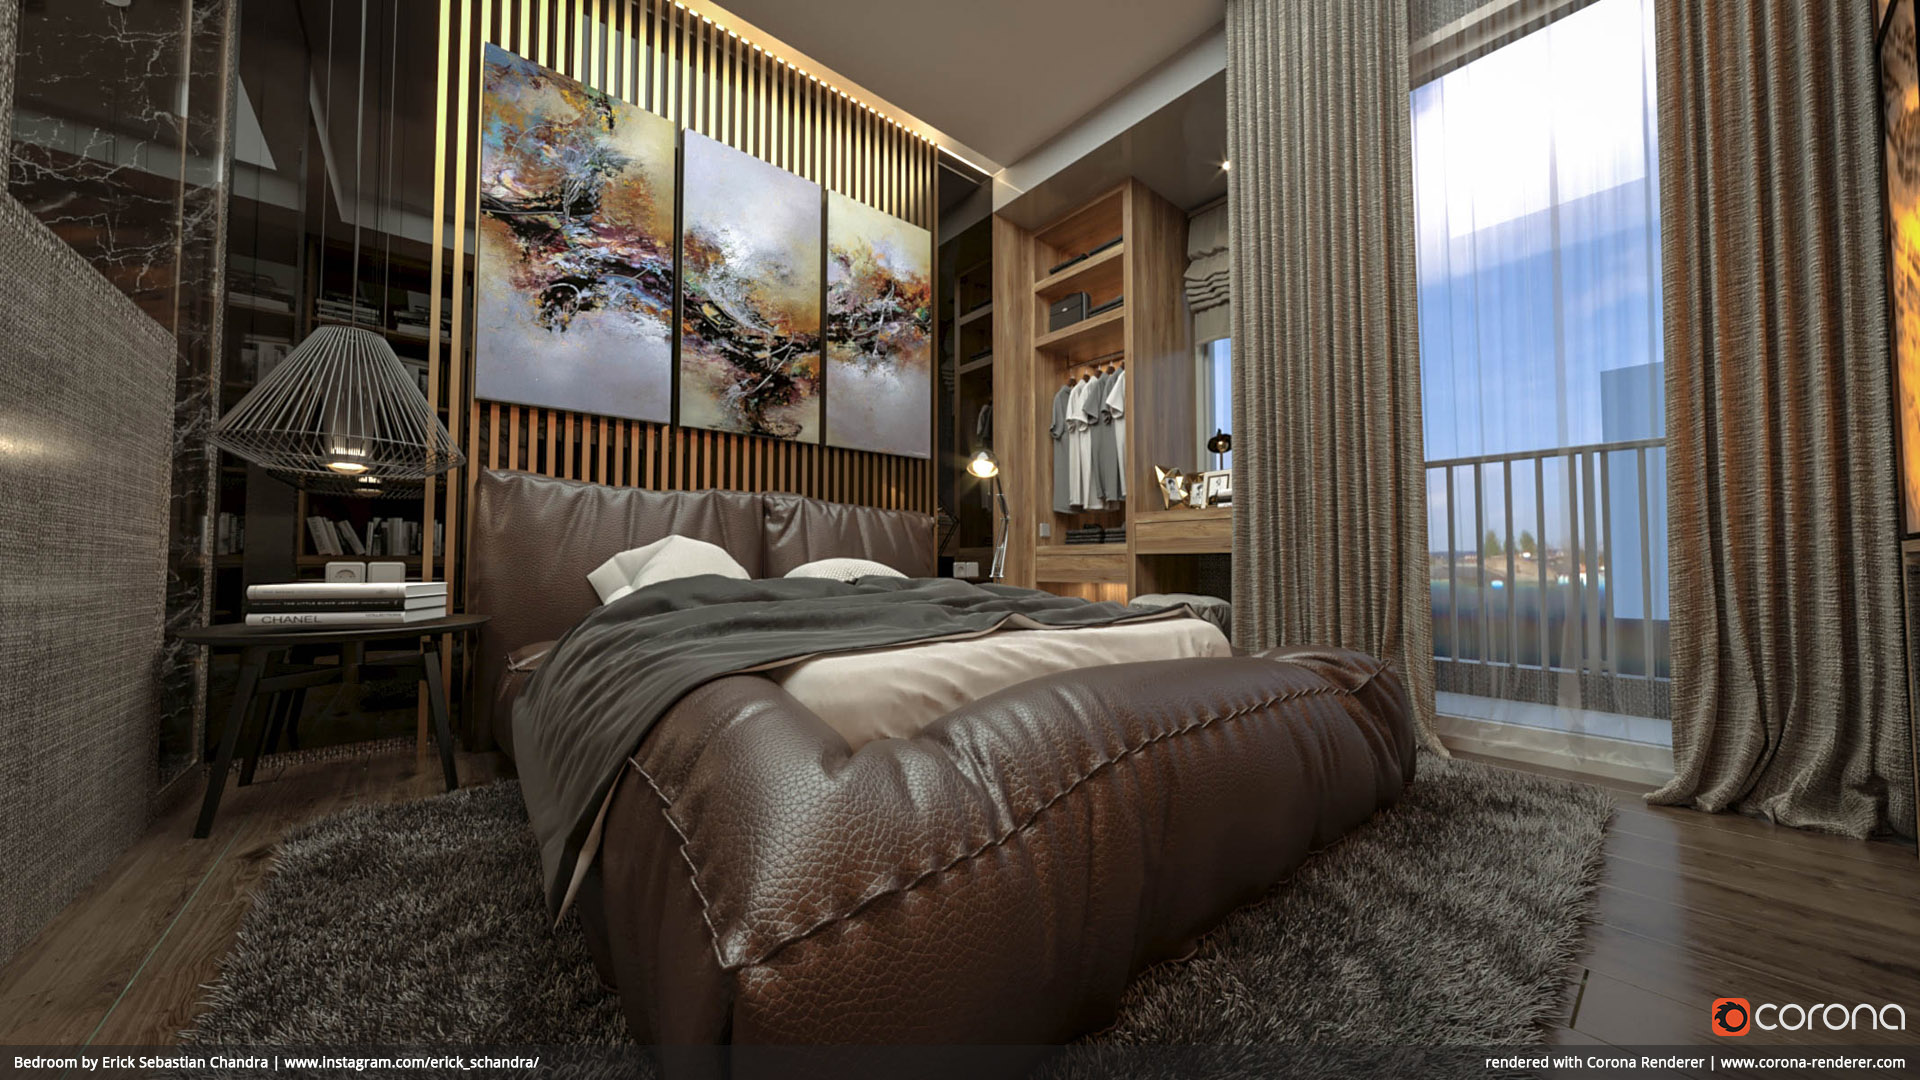
\includegraphics[width=\linewidth]{img/corona_render.jpg}
	\caption{An image generated with the Corona Renderer}
	\label{fig:corona_render}
\end{figure}

The main idea is similar for every renderer:
\begin{enumerate}
	\item A 3D digital scene is described by the objects it contains
	\item A light simulation algorithm runs for every visible pixel from the viewer
	\item Upon object interaction, the shading of the intersected point is computed
	\item When it's done, results in form of a picture ("photograph") called \emph{render} are created
\end{enumerate}

Please see figure ~\ref{fig:path_tracer} for a simple demonstration of this workflow.

\begin{figure}[H]
	\centering
	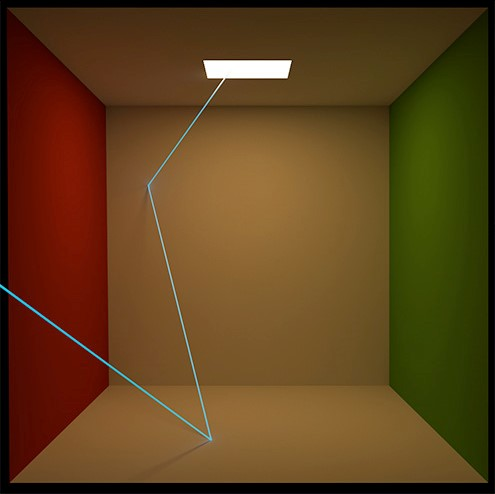
\includegraphics[width=85mm]{img/path_tracer.jpg}
	\caption{A visualization of a light transport algorithm (path tracer)~\cite{mitsubaWeb}}
	\label{fig:path_tracer}
\end{figure}

\subsection{Digital scene}

The basic elements of a digital scene are roughly the same for each renderer. 

\begin{description}
	\item[Camera] A camera in a digital scene works in the same manner as in real life --- it records a picture. Generally, you may define the coordinate position and the viewing vectors but also the properties such as focal distance or the type of film.
	\item[Light source] The scene needs to be illuminated by one or multiple sources in order to be visible. The common kinds of lights are point light, area light, spot light or environment (constant) lighting. 
	\item[Objects] The actual visible content of the scene are objects. Almost all rendering systems offer a choice to either use their precomputed basic geometry such as spheres or triangles or to include a mesh geometry described in an external file (usually created by modeling software). They also have to state their material properties so that the algorithm may correctly interact with them, e.g. diffuse vs. reflective material.
\end{description}

Unfortunately, as each renderer may have a very unique implementation details, the formats of the scenes are vastly different. For example, mitsuba uses XML but PBRT has its own specific format. An example of a simple scene for Mitsuba2 can be found in \ref{fig:example_scene}.

\definecolor{maroon}{rgb}{0.5,0,0}
\definecolor{darkgreen}{rgb}{0,0.5,0}
\lstdefinelanguage{XML}
{
	basicstyle=\ttfamily,
	morestring=[s]{"}{"},
	morecomment=[s]{?}{?},
	morecomment=[s]{!--}{--},
	commentstyle=\color{darkgreen},
	moredelim=[s][\color{black}]{>}{<},
	moredelim=[s][\color{red}]{\ }{=},
	stringstyle=\color{blue},
	identifierstyle=\color{maroon}
}

\begin{figure}[httpb]
\begin{tabular}{p{0.3\textwidth}p{0.6\textwidth}}
\begin{minipage}{0.3\textwidth}
	
\includegraphics[width=\linewidth]{img/example_scene.png}
\end{minipage}
	&
\begin{minipage}{0.6\textwidth}
	\lstset{language=XML}
	\begin{lstlisting}[basicstyle=\tiny]
<scene version="2.0.0">
 <!-- Light transport algorithm -->
 <integrator type="path"/>
	
 <!-- Camera looking at the sphere -->
 <sensor type="perspective">
  <transform name="to_world">
   <lookat origin="0,-6,0" target="0,0,0" up="0,0,1"/>
  </transform>
 </sensor>
	
 <!-- Red sphere in the middle -->
 <shape type="sphere">
  <bsdf type="diffuse">
   <rgb name="reflectance" value="1.0,0.0,0.0"/>
  </bsdf>
 </shape>
	
 <!-- Light blue light all around the scene-->
 <emitter type="constant">
  <rgb name="radiance" value="0.6,0.8,0.9"/>
 </emitter>
</scene>
	\end{lstlisting}
\end{minipage}
\end{tabular}
\label{fig:example_scene}
\caption{A simple scene rendered with Mitsuba2 (left) along with its scene descriptiont (right)}
\end{figure}

\subsection{Light simulation}

The fundamental part of the rendering process is its implementation of the light transport simulation. The following sections will describe the theory and the physics models that are behind the light transport and then we look at the specific algorithms. 

\subsubsection{BRDF}

The materials of objects inside a scene are described by \emph{Bidirection Distrubtion Reflectance Function}, shortly \emph{BRDF}. This function is given the incoming vector $\omega_i$, the outgoing vector $\omega_o$ and it tells us how much radiance is reflected from the direction $\omega_i$ to the direction $\omega_o$. By the definition~\cite{nicodemus1965directional}, it looks as follows:

\begin{equation}
f_r(\omega_i,\omega_o)=\frac{dL_o(\omega_o)}{L_i(\omega_i)cos\theta_i d\omega_i}
\end{equation}

The function is shown in \ref{fig:brdf}. As it is a distribution function, we can rather describe it as a probability density that a defined amount of light energy gets reflected from $\omega_i$ to $\omega_o$.

\begin{figure}[H]
	\centering
	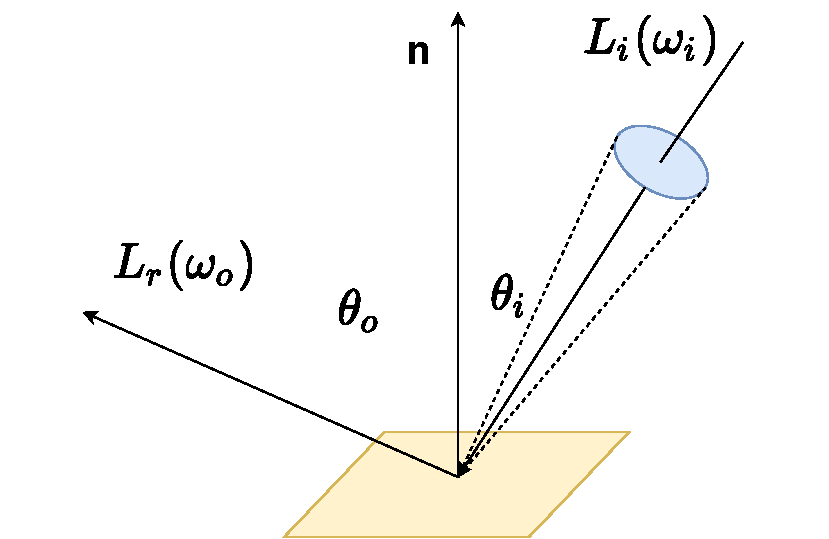
\includegraphics[width=85mm]{img/brdf.pdf}
	\caption{A Bidirectional Distribution Reflectance Function}
	\label{fig:brdf}
\end{figure}

In the simplest cases this states how reflective the surface of an object is. A comparison between diffuse and reflective BRDFs is displayed in 

\begin{figure}[H]
	\centering
	\begin{minipage}{.5\textwidth}
		\centering
		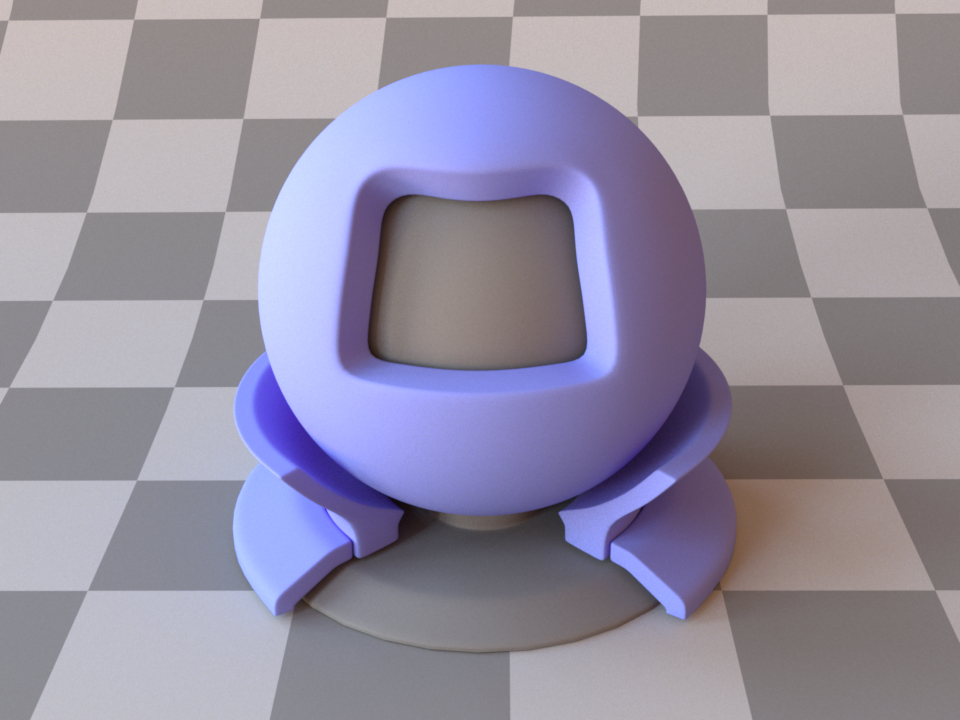
\includegraphics[width=.9\linewidth]{img/bsdf_diffuse.jpg}
	\end{minipage}%
	\begin{minipage}{.5\textwidth}
		\centering
		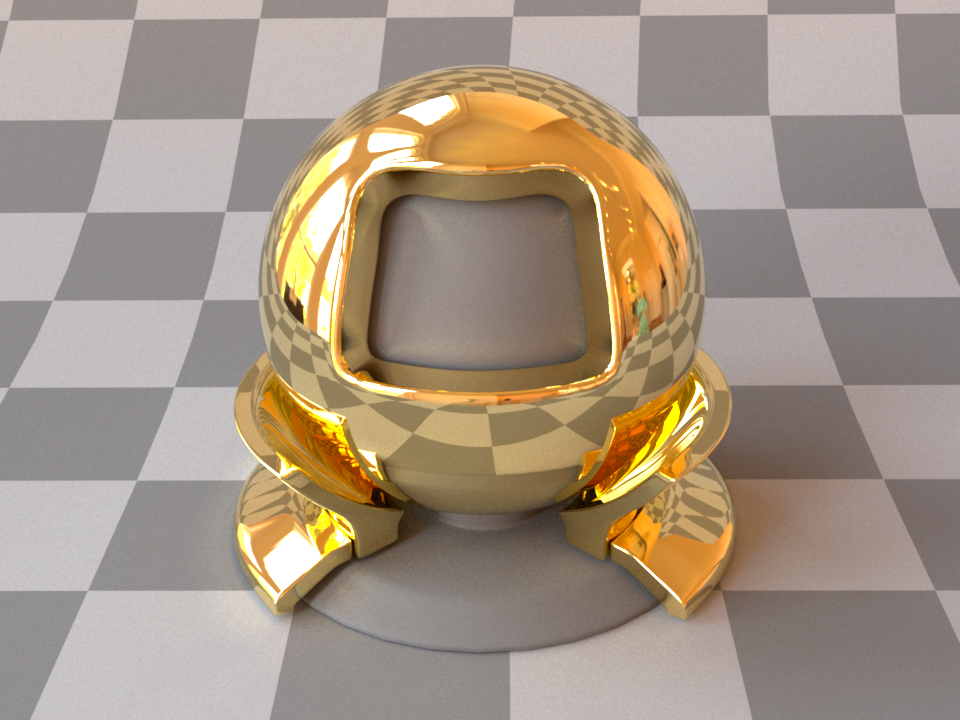
\includegraphics[width=.9\linewidth]{img/bsdf_reflective.jpg}
	\end{minipage}
\caption{Diffuse (left) and reflective gold (right) by Mitsuba2~\cite{mitsubaWeb}}
\label{fig:diffuse_reflective}
\end{figure}

Physically based BRDFs must fulfill several properties~\citealp{duvenhage2013numerical}:
\begin{description}
	\item[Heimholtz reciprocity] The amount of reflected energy from the incoming direction to the outgoing direction is equal to the amount of energy in the reversed directions ($f_r(\omega_i,\omega_o)=f_r(\omega_o,\omega_i)$)
	\item[Energy conservation] The amount of reflected energy cannot be larger than received
	\item[Positivity] BRDF is always positive ($f_r(\omega_i,\omega_o)\le0$)
\end{description}

Note that BRDF concerns only opaque surfaces. There exist multiple distribution functions that describe behavior of other materials, for example:
\begin{description}
	\item[BTDF] Describes light transmission
	\item[BSDF] Combination of BTDF and BRDF (e.g. glass, water)
	\item[BSSRDF] Considers scattering of the light under the surface as well (skin)
\end{description}


\subsubsection{Rendering equation}

The physically based realistic rendering is in reality an approach to solve some of the formulations of the \emph{rendering equation}~\cite{kajiya1986rendering}. It looks as follows:

\begin{equation}
L_o(x,\omega_o)=L_e(x,\omega_o)+\int_{\Omega}f_r(x,\omega_o,\omega_i) L_i(x,\omega_,i) cos\theta_i d\omega_i
\end{equation}




